\iffalse 
\documentclass[journal,12pt,twocolumn]{IEEEtran}
\usepackage{graphicx}
\graphicspath{{./figs/}}{}
\usepackage{amsmath,amssymb,amsfonts,amsthm}
\newcommand{\myvec}[1]{\ensuremath{\begin{pmatrix}#1\end{pmatrix}}}

\let\vec\mathbf

\title{
Matrix-Lines
}
\author{R.Radhika}
\begin{document}
\maketitle
\tableofcontents
\bigskip
\section{Problem Statement}
\fi
\\
\solution 
	\begin{figure}[!ht]
		\centering
 \includegraphics[width=\columnwidth]{chapters/11/10/1/12/figs/figure.pdf}
		\caption{}
		\label{fig:11/10/1/12}
  	\end{figure}
\iffalse
\section{Construction}
\begin{figure}[h]
    \centering
\includegraphics[width=\columnwidth]{figure.pdf}
    \caption{Equation of the slope}
    \label{fig:my_label}
\end{figure}
\vspace{2cm}
\begin{table}[h]
    \centering
    \begin{tabular}{|c|c|c|}
       \hline
       \textbf{Symbol}&\textbf{Value}&\textbf{Description}  \\
       \hline
	    $\vec{A}$ & $\myvec{
		    x_1\\
		    y_1}$
	    & Point on X-axis\\
        \hline
	    $\vec{B}$ & $\myvec{h\\k}$
 & Point on Y-axis\\
        \hline
        \hline
        A & k-y1=m(h-x1) & Given Condition\\
        \hline
    \end{tabular}
    \caption{Parameters}
    \label{tab:my_label}
\end{table}


\section{Solution}
Given that resultant line passes through point(x1,y1) and (h,k) (let prove the equation in vector form by line eqation ) \\
\\
\\
\fi
Given 
\begin{align}
\vec{A}=\myvec{
  x_1\\
  y_1}
 , \vec{B}=\myvec{
  h\\
  k}
\end{align}

\iffalse
\textbf{First Method}:\\
condition is	
\begin{equation}
	{\vec{n^{\top}}\vec{{m}}} = 0 \\     \label{eq-1}
\end{equation}	
m is 
\fi
The direction vector
\begin{align}
	\vec{m} &= \vec{B}-\vec{A}
	\\
	&=
	\myvec{
  h-x_1\\
  k-y_1
  }
   \equiv
	\myvec{
1\\
	\frac{ k-y_1}{h-x_1}
  }
\end{align}
which yields the desired relation from 
		\eqref{eq:two-dir-vec}.
\iffalse
\begin{equation}
 			\myvec{
					-m& 1}\myvec{
  h-x_1\\
  k-y_1
  }
   = 0  \label{eq-4}
\end{equation}
by solving eq-4
\begin{equation}
	\myvec{
 -m (h-x_1))+(k-y_1}=0
\end{equation}
Then the equation becomes\\

$\myvec{
  k-y_1)=m(h-x_1}$\\
Therefore the Resultant Equation of line is\\
\begin{equation}
	\myvec{
  k-y_1)=m(h-x_1}
\end{equation}
\begin{table}[h]
    \centering
    \begin{tabular}{|c|}
    \hline \\
           \myvec{
  k-y_1)=m(h-x_1}\\
         \\
\hline
    \end{tabular}
\end{table}\\
\textbf{Second Method}:\\
given ${\vec{A}}$=$\myvec{
  x_1\\
  y_1}$
  ${\vec{B}}$=$\myvec{
  h\\
  k}$\\
C=$\myvec{
  \frac{x_1+h}{2}\\
  \frac{y_1+k}{2}
}$\\
m is the direction vector\\

		 m=C-A\\
		 
		 m=B-C\\
		 		 
m=$\myvec{
  \frac{x_1+h}{2}-x_1\\
  \frac{y_1+k}{2}-y_1
}$\\

 m=2$\myvec{
  \frac{h-x_1}{2}\\
  \frac{k-y_1}{2}
}$\\

m=$\myvec{
  {h-x_1}\\
  {k-y_1}
}$\\

condition is	
\begin{equation}
	{\vec{n^{\top}}\vec{{m}}} = 0 \\     \label{eq-1}
\end{equation}
\begin{equation}
 			\myvec{
					-m& 1}\myvec{
  h-x_1\\
  k-y_1
  }
   = 0  \label{eq-4}
\end{equation}
by solving eq-4
\begin{equation}
	\myvec{
 -m (h-x_1))+(k-y_1}=0
\end{equation}
Then the equation becomes\\

$\myvec{
  k-y_1)=m(h-x_1}$\\
Therefore the Resultant Equation of line is\\
\begin{equation}
	\myvec{
  k-y_1)=m(h-x_1}
\end{equation}			 


\textbf{Third Method}:\\
\begin{equation}
	{\vec{n^{\top}}\vec{{m}}} = 0 \\     \label{eq-1}
\end{equation}		
\begin{equation}
	{\vec{n^{\top}}\vec{({x}-A)}} = 0 \\     \label{eq-2}
\end{equation}
\begin{equation}
	{\vec{n^{\top}}\vec{({x}-B)}} = 0      \label{eq-3}
\end{equation}


 The Equation of line through ${\vec{A}}$  from 1 is\\
\begin{equation}
	\vec{n^{\top}}\myvec{ 
	\myvec{
  x\\
  y}
  - \label{eq-4}
	\myvec{
  x_1\\
  y_1}}
   = 0 \
\end{equation}
\\
Equation of line passing through ${\vec{B}}$ from 2 is\\
\begin{equation}
	\vec{n^{\top}}\myvec{ 
	\myvec{
  x\\
  y}
  - \label{eq-5}
	\myvec{
  h\\
  k}}
  = 0 \
\end{equation}
\\
Now by solving eq3,\\
\begin{equation}
	\vec{n^{\top}}
	\myvec{
  x-x_1\\
  y-y_1
}
  = 0 \label{eq-6}
\end{equation}
 
Now by solving eq4,\\
\begin{equation}
	\vec{n^{\top}}
	\myvec{
  x-h\\
  y-k
}
  = 0 \label{eq-7}
\end{equation}
 \\
 From eq5 and eq6 we can prove the equation ${\vec{n}}$,\\
 \\
 \begin{equation}
 			\myvec{
					-m& 1}\myvec{
  x-x_1& y-y_1\\
  x-h & y-k
 }
	 = 0   \
\end{equation}\\
 by solving 7 th equation\\
 \begin{equation}
	\myvec{
  k-y_1)=m(h-x_1}
\end{equation}
\\
Therefore the Resultant Equation of line is ${\vec{n^{\top}}\vec{X}} = c$ 
\\
 \begin{equation}
	\myvec{
  k-y_1)=m(h-x_1}
\end{equation}

\section{Software}
Download the following code using,
\begin{table}[h]
    \centering
    \begin{tabular}{|c|}
    \hline \\
         https://github.com/Radhikarkv/fwcproject.git  \\
         \\
\hline
    \end{tabular}
\end{table}
\\
and execute the code by using command
\begin{center}
\textbf{Python3 lineassign.py}\\
\end{center}

\section{Conclusion}
prove the equation of a line passes trough a points$(x_1,y_1)$,(h,k) if slope of the line is m i.e $(k-y_1)=m(h-x_1)$.

\end{document}
\fi
